\documentclass[12pt,compress,aspectratio=169]{beamer}

\mode<presentation>
{
  \usetheme{Singapore}
  \setbeamersize{text margin left=1cm,text margin right=1cm}
%  \setbeamertemplate{navigation symbols}{} % suppress nav bar
%  \setbeamercovered{transparent}
}
\usefonttheme{professionalfonts}
\usepackage{amsmath,bm}
\usepackage{siunitx}
%\usepackage{graphicx}
\usepackage{tikz}
\usepackage{mathpazo}
\usepackage[scaled]{helvet}
%\usepackage{xcolor,colortbl}
%\usepackage{hyperref}

\sisetup{number-math-rm=\mathnormal}

\title{Class 5: Circular Motion}
\subtitle{AP Physics}
\author[TML]{Timothy Leung, Ph.D.}
\institute{Olympiads School}
\date{Fall/Winter 2017}

\newcommand{\pic}[2]{\includegraphics[width=#1\textwidth]{#2}}
\newcommand{\mb}[1]{\ensuremath\mathbf{#1}}

\begin{document}

\begin{frame}
  \maketitle
\end{frame}

\begin{frame}
  \frametitle{Files to Download}
  \framesubtitle{Please download/print the PDF file}
  \begin{itemize}
%  %\item\texttt{00-outline.pdf}--The course outline (slightly updated)
  \item\texttt{05-rotMotion-print.pdf}--The ``print version'' of this week
    and next week's slides. I recommend printing 4 slides per page.
  \item\texttt{0506-Homework.pdf} This week's homework.
%    We are taking up questions from Class 3 today, but please hand in Classes 3
%    \& 4 homework together next week.
  \end{itemize}
\end{frame}


\begin{frame}
  \frametitle{Today's Plan}
  \begin{enumerate}
  \item Take up questions from Classes 3 and 4 homework
  \item Go over this week's slides (it will take more than one day)
  %\item Time permitting: take up questions from Class 1 and 2 (calculus)
  \end{enumerate}
\end{frame}


\section{Polar Coordinates}
\begin{frame}
  \frametitle{Polar Coordinate System}
  \begin{columns}
    \column{.28\textwidth}
    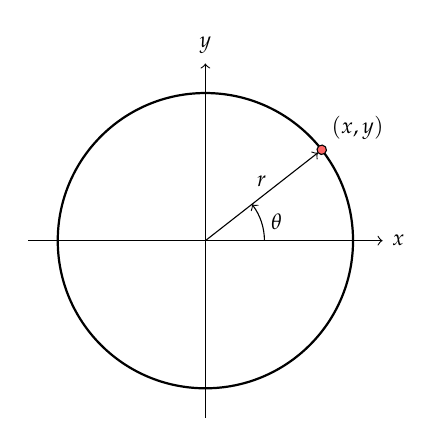
\begin{tikzpicture}[scale=0.75]
      \draw[->](-3,0)--(3,0) node[pos=1,right]{\footnotesize$x$};
      \draw[->](0,-3)--(0,3) node[pos=1,above]{\footnotesize$y$};
      \draw[thick] (0,0) circle(2.5);
      \begin{scope}[rotate=38]
        \draw[->] (0,0)--(2.42,0) node[midway,above]{\footnotesize$r$};
        \draw[fill=red!60] (2.5,0) circle(0.08)
        node[above right]{\footnotesize$(x,y)$};
      \end{scope}
      \draw(1,0)[->] arc(0:38:1) node[midway,right]{\footnotesize$\theta$};
    \end{tikzpicture}
    \column{.7\textwidth}
    \begin{itemize}
    \item Cartesian system $\mb{x}(x,y)$ is not the only option!
    \item For circular motion, \textbf{polar coordinates} are better
    \item Position described by $\mb{r}(r,\theta)$
      \begin{itemize}
      \item $r$ is distance from the origin
      \item $\theta$ standard angle
      \end{itemize}
%      \vspace{-0.2in}{\large
%        \begin{displaymath}
%          \mb{r}=r\hat{\bm{r}}+\theta\hat{\bm{\theta}}
%        \end{displaymath}
%      }
    \item Cartesian coordinates are related to the polar coordinates by:

      \vspace{-0.45in}{\large
        \begin{align*}
          x&=r\cos\theta\\
          y&=r\sin\theta
        \end{align*}
      }
    \item In 3D, $z$ coordinates of both Cartesian and polar systems
      are the same
    \end{itemize}
  \end{columns}
\end{frame}


\begin{frame}
  \frametitle{Rigid Body Motion}
  \framesubtitle{Angular Position and Angular Velocity}
  \begin{columns}
    \column{.28\textwidth}
    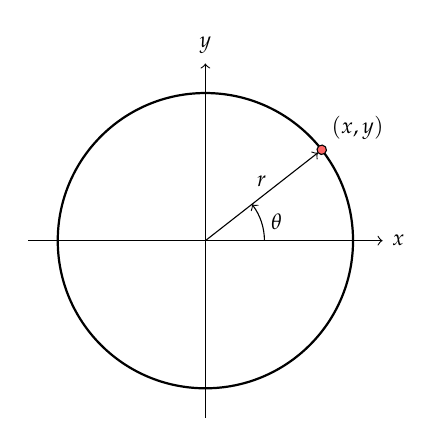
\begin{tikzpicture}[scale=0.75]
      \draw[->](-3,0)--(3,0) node[pos=1,right]{\footnotesize$x$};
      \draw[->](0,-3)--(0,3) node[pos=1,above]{\footnotesize$y$};
      \draw[thick] (0,0) circle(2.5);
      \begin{scope}[rotate=38]
        \draw[->] (0,0)--(2.42,0) node[midway,above]{\footnotesize$r$};
        \draw[fill=red!60] (2.5,0) circle(0.08)
        node[above right]{\footnotesize$(x,y)$};
      \end{scope}
      \draw(1,0)[->] arc(0:38:1) node[midway,right]{\footnotesize$\theta$};
    \end{tikzpicture}
    \column{.7\textwidth}
    \begin{itemize}
    \item For constant $r$, \textbf{angular position} $\theta$ determines an
      object's position as a function of time:
      
      \vspace{-0.2in}{\large
        \begin{displaymath}
          \boxed{\theta=\theta(t)}
        \end{displaymath}
      }
    \item\textbf{Angular velocity} $\omega$ (or \textbf{angular frequency})
      is its time derivative
      
      \vspace{-0.3in}{\large
        \begin{displaymath}
          \boxed{\omega=\frac{d\theta(t)}{dt}}
        \end{displaymath}
      }
    \item $\theta$ is measured in \si{radians}, and $\omega$ in \si{rad/\s}
    \item e.g.\ an object rotating at one revolution per second has an angular
      velocity of $\omega=\SI{2\pi}{/\s}$
    \end{itemize}
  \end{columns}
\end{frame}

\begin{frame}
  \frametitle{Rigid Body Motion}
  \framesubtitle{Angular Velocity}
  \begin{columns}
    \column{.28\textwidth}
    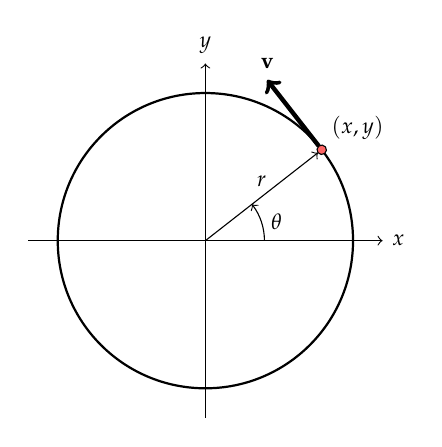
\begin{tikzpicture}[scale=0.75]
      \draw[->](-3,0)--(3,0) node[pos=1,right]{\footnotesize$x$};
      \draw[->](0,-3)--(0,3) node[pos=1,above]{\footnotesize$y$};
      \draw[thick] (0,0) circle(2.5);
      \begin{scope}[rotate=38]
        \draw[->] (0,0)--(2.42,0) node[midway,above]{\footnotesize$r$};
        \draw[fill=red!60] (2.5,0) circle(0.08)
        node[above right]{\footnotesize$(x,y)$};
        \draw[ultra thick,->](2.5,0.08)--(2.5,1.5)
        node[pos=1,above]{\footnotesize$\mb{v}$};
      \end{scope}
      \draw(1,0)[->] arc(0:38:1) node[midway,right]{\footnotesize$\theta$};
    \end{tikzpicture}
    \column{.7\textwidth}
    \begin{itemize}
    \item Speed $v$ and $\omega$ are related simply by:

      \vspace{-0.35in}{\Large
        \begin{displaymath}
          \boxed{v=r\omega}
        \end{displaymath}
      }
    \item Or in vector form:

      \vspace{-0.35in}{\Large
        \begin{displaymath}
          \boxed{\mb{v}=\bm{\omega}\times\mb{r}}
        \end{displaymath}
      }
    \item $\mb{v}$ is always tangent to circle (perpendicular to $\mb{r}$)
    \item We can also relate $\omega$ to \textbf{frequency} and \textbf{period}
      of the rotation:

      \vspace{-0.4in}{\Large
        \begin{displaymath}
          \boxed{f=\frac{\omega}{2\pi}}\quad
          \boxed{T=\frac{2\pi}{\omega}}\quad
          \boxed{f=\frac{1}{T}}
        \end{displaymath}
      }
      
      \vspace{-0.1in}$T$ is in seconds (\si{\s}) and $f$ is in hertz
      (\si{\hertz})
    \end{itemize}
  \end{columns}
\end{frame}


\begin{frame}
  \frametitle{Rotating Object Without Slipping}
  A tire with radius $r$ rolls along the road with an angular velocity $\omega$
  \emph{without slipping}. (This is a very common case for analysis.)  What
  is its velocity $v$
  \begin{enumerate}[a.]
  \item at the contact between the ground and the tire?
  \item at the center?
  \item at the top of the tire?
  \end{enumerate}
  \vspace{-0.4in}
  \begin{center}
    \hspace{1in}
    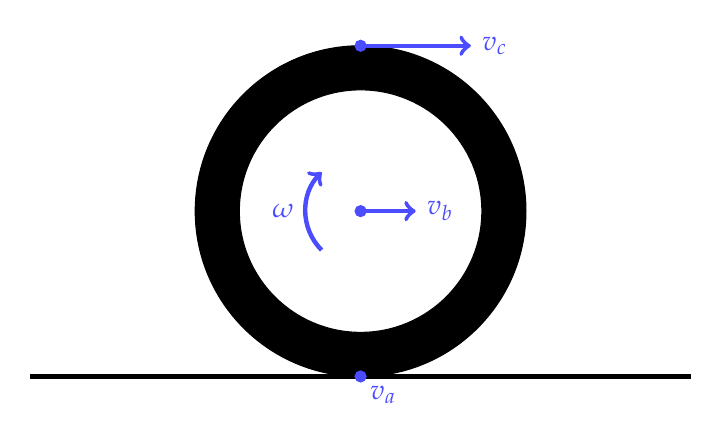
\begin{tikzpicture}[scale=0.7]
      \draw[fill=black](0,0) circle(3);
      \draw[fill=white](0,0) circle(2.2);
      \draw[ultra thick](-6,-3)--(6,-3);
      \draw[ultra thick,blue!70,->](-0.707,-0.707) arc(225:135:1)
      node[midway,left]{$\omega$};
      \draw[fill=blue!70,blue!70](0,-3) circle(0.1) node[below right]{$v_a$};
      \draw[fill=blue!70,blue!70](0,0) circle(0.1);
      \draw[ultra thick,blue!70,->](0,0)--(1,0) node[pos=1,right]{$v_b$};
      \draw[fill=blue!70,blue!70](0,3) circle(0.1);
      \draw[ultra thick,blue!70,->](0,3)--(2,3) node[pos=1,right]{$v_c$};
    \end{tikzpicture}
  \end{center}
\end{frame}

\begin{frame}
  \frametitle{Rigid Body Motion}
  \framesubtitle{Angular Acceleration}
  \begin{itemize}
  \item The derivative of $\omega$ with respect to time gives us
    \textbf{angular acceleration}:

    \vspace{-0.2in}{\Large
      \begin{displaymath}
        \boxed{\alpha=\frac{d\omega(t)}{dt}=\frac{d^2\theta(t)}{dt^2}}
      \end{displaymath}
    }

    \vspace{-0.1in}$\alpha$ has the unit of \si{rad/\sec^2}.

  \item For \emph{uniform} circular motion, $\omega$ is constant, and $\alpha=0$
  \item Not surprisingly, \textbf{tangential acceleration} is related to
    angular acceleration by the radius $r$
    
    \vspace{-0.2in}{\Large
      \begin{displaymath}
        \boxed{a_\theta=\frac{dv}{dt}=r\frac{d\omega(t)}{dt}=r\alpha}
      \end{displaymath}
    }

  \end{itemize}
\end{frame}


\begin{frame}
  \frametitle{Kinematics in the Angular Direction}
  \framesubtitle{These Should Look Familiar}
  For constant $\alpha$, the kinematic equations are just like in linear
  motion:
  
  \begin{columns}
    \column{0.55\textwidth}
    {\LARGE
      \begin{align*}
        \Delta\theta&=\omega_1\Delta t + \frac{1}{2}\alpha\Delta t^2\\
        \Delta\theta&=\omega_2\Delta t - \frac{1}{2}\alpha\Delta t^2
      \end{align*}
    }
    \column{0.45\textwidth}
    {\LARGE
      \begin{align*}
        \Delta\theta&=\frac{\omega_1+\omega_2}{2} \Delta t\\
        \omega_2&= \omega_1+ \alpha\Delta t\\
        \omega_2^2& = \omega_1^2+ 2\alpha\Delta\theta
      \end{align*}
    }
  \end{columns}
  Of course, if $\alpha$ is \emph{not} non-constant, we will have to integrate
\end{frame}


\begin{frame}
  \frametitle{A Simple Example}
  \textbf{Example 1:} An object moves in a circle with angular acceleration
  \SI{3}{rad/\s^2}. The radius is \SI{2}{\metre} and it starts from rest. How
  long it takes for this object to finish a circle?
\end{frame}


\begin{frame}
  \frametitle{Nothing is Ever \emph{That} Simple}
  \begin{itemize}
  \item Remember, even when $\alpha=0$, we still have a centripetal
    acceleration $a_r$ for any circular motion

    \vspace{-0.1in}{\large
      \begin{displaymath}
        \boxed{a_r=\frac{v^2}{r}=\omega^2r=\frac{4\pi^2r}{T}=4\pi^2rf}
      \end{displaymath}
    }

  \item And with the acceleration, there is always a \textbf{centripetal force}

    \vspace{-0.1in}{\large
      \begin{displaymath}
        \boxed{F_r=ma_r=\frac{mv^2}{r}}
      \end{displaymath}
    }
  \end{itemize}
\end{frame}


\begin{frame}
  \frametitle{Acceleration: The General Case}
  \begin{columns}
    \column{0.2\textwidth}
    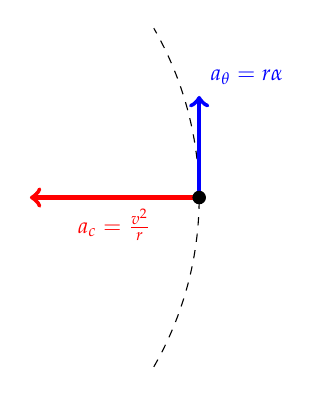
\begin{tikzpicture}[scale=4.3]
      %\draw[dashed] (0,0) circle(3);
      \draw[dashed] (0.866,-0.5) arc(-30:30:1);
      \draw[ultra thick, red,->] (1,0)--(0.5,0)
      node[pos=0.5,below]{\footnotesize $a_c=\frac{v^2}{r}$};
      \draw[ultra thick, blue,->] (1,0)--(1,0.3)
      node[pos=1,above right]{\footnotesize $a_\theta=r\alpha$};
      \fill (1,0) circle(0.02);
    \end{tikzpicture}
    \column{0.8\textwidth}
    \begin{itemize}
    \item In general circular motion, there are two components of acceleration:
      \begin{itemize}
      \item\textcolor{red}{\textbf{Centripetal acceleration} $a_c$} depends on
        radius of curvature $r$ and speed $v$
      \item \textcolor{blue}{\textbf{Tangential acceleration} $a_\theta$}
        depends on radius $r$  and angular acceleration $\alpha$
      \end{itemize}
    \item Fortunately, most of the cases in AP Physics are uniform circular
      motion
    \end{itemize}
  \end{columns}
\end{frame}


\begin{frame}
  \frametitle{How to Solve Circular Motion Problems}

  A two-step process:
  \begin{enumerate}
  \item Is there any circular motion?
  \item If so, the condition for circular motion is:

    \vspace{-0.2in}{\Large
      \begin{displaymath}
        \mb{F}_\mathrm{provided}=\mb{F}_\mathrm{required}
      \end{displaymath}
    }
    \begin{itemize}
    \item The \emph{provided} force comes from FBD
    \item The \emph{required} force comes from the centripetal equation we have
    \end{itemize}
  \end{enumerate}
\end{frame}


\begin{frame}
  \frametitle{Example: Horizontal Motion}
  \begin{columns}
    \column{0.4\textwidth}
    \pic{1}{puck-on-table.jpg}
    \column{0.6\textwidth}
    \textbf{Example 2:} In the figure on the left, a mass $m_1=\SI{3}{\kg}$ is
    rolling around a frictionless table with radius $R=\SI{1}{\metre}$. with a
    speed of \SI{2}{\metre/s}. What is the mass of the weight $m_2$?
  \end{columns}
\end{frame}


\begin{frame}
  \frametitle{Another Example: Exit Ramp}
  \textbf{Example 3:} A car exits a highway on a ramp that is banked at
  \ang{15} to the horizontal. The exit ramp has a radius of curvature of
  \SI{65}{\metre}. If the conditions are extremely icy and the driver cannot
  depend on any friction to help make the turn, at what speed should the driver
  travel so that the car will not skid off the ramp? What if there is friction?
\end{frame}


\begin{frame}
  \frametitle{Vertical Circles}
  \begin{itemize}
  \item Uniform circular motion with a horizontal path is straightforward
  \item For vertical motion:
    \begin{itemize}
    \item Generally not solvable by dynamics
    \item We can use conservation of energy to solve for $\mb{v}$
    \item Then use the equation for centripetal force to find other forces
    \item\textbf{Remember: } If it is impossible to get the required
      centripetal force, then it could not continue the circular motion
    \end{itemize}
  \end{itemize}
\end{frame}


\begin{frame}
  \frametitle{Example}
  \textbf{Example 4:} A cord is tied to a pail of water, and the pail is swung
  in a vertical circle of \SI{1}{\metre}. What must be the minimum velocity of
  the pail be at its highest point so that no water spills out?

  \begin{enumerate}[(a)]
  \item\SI{3.1}{m/\s}
  \item\SI{5.6}{m/\s}
  \item\SI{20.7}{m/\s}
  \item\SI{100.5}{m/\s}
  \end{enumerate}
\end{frame}


\begin{frame}
  \frametitle{Example: Roller Coaster}
  \textbf{Example 5:} A roller coaster car is on a track that forms a circular
  loop, of radius $R$, in the vertical plane. If the car is to maintain contact
  with the track at the top of the loop (generally considered to be a good
  thing), what is the minimum speed that the car must have at the bottom of the
  loop. Ignore air resistance and rolling friction.

  \begin{enumerate}[(a)]
  \item $\sqrt{2gR}$
  \item $\sqrt{3gR}$
  \item $\sqrt{4gR}$
  \item $\sqrt{5gR}$
  \end{enumerate}
\end{frame}


\begin{frame}
  \frametitle{Example}
  \textbf{Example 6:} A stone of mass $m$ is attached to a light strong string
  and whirled in a \emph{vertical} circle of radius $r$. At the exact bottom of
  the path, the tension of the string is three times the weight of the stone.
  The stone's speed at that point is given by:
  \begin{enumerate}[(a)]
  \item $2\sqrt{gR}$
  \item $\sqrt{2gR}$
  \item $\sqrt{3gR}$
  \item $4gR$
  \end{enumerate}
\end{frame}


\section{Torque}


\begin{frame}
  \frametitle{Torque and Rotational Equilibrium}
  Let's consider this question:

  \begin{center}
    \fbox{
      \begin{minipage}{0.7\textwidth}
        Two people stand on a board of uniform density. One person has a mass of
        \SI{50}{\kg} and stands \SI{10}{\metre} away from the fulcrum (pivot).
        The second person has a mass of \SI{65}{\kg}. How far away from the
        fulcrum would the second person have to stand for the system to have
        to be in equilibrium?
      \end{minipage}
    }
  \end{center}
\end{frame}

\begin{frame}
  \frametitle{Equation of Motion}
  \framesubtitle{Newton's Second Law}
  \begin{itemize}
  \item Newton's 2nd Law of motion:
    
    \vspace{-0.3in}{\LARGE
    \begin{displaymath}
      \mb{F}_\mathrm{net}=m\mb{a}
    \end{displaymath}
  }
  \item Is it also true for \emph{circular} motion?
  \item If a net force $\mb{F}_\mathrm{net}$ causes a mass to accelerate
    (linearly), what causes a mass to go into circular motion?
  \end{itemize}

  \uncover<2->{
    \vspace{0.3in}
    \textbf{Answer: } We need to introduce a few concepts first\ldots
  }
\end{frame}

\begin{frame}
  \frametitle{Torque (Moment)}
  I have a pencil sitting on a table, and with my fingers, I push the two ends
  of the pencil with equal force $\textcolor{red}{F}$. \textbf{What happens?}
  \begin{center}
    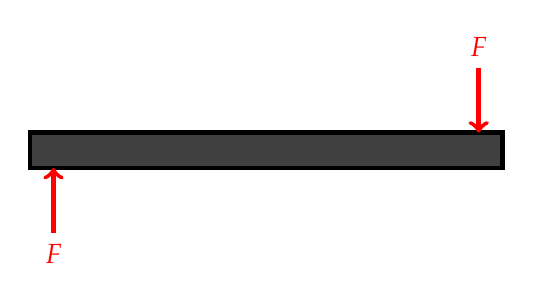
\begin{tikzpicture}[scale=1.5]
      \fill[black!75,draw=black,ultra thick] (-2,-0.15) rectangle (2,0.15);
      \draw[ultra thick,red,->](-1.8,-.7)--(-1.8,-.15) node[pos=0,below]{$F$};
      \draw[ultra thick,red,->]( 1.8,0.7)--( 1.8,0.15) node[pos=0,above]{$F$};
    \end{tikzpicture}
  \end{center}
  $\mb{F}_\mathrm{net}=\mb{0}$, therefore $\mb{a}=\mb{0}$. But (obviously) it
  won't stay still either!
\end{frame}


\begin{frame}
  \frametitle{What is Torque?}
  \begin{itemize}
  \item The tendency of a force to cause or change the rotational motion of a
    body.
  \item A force acting at a point some distance from a fulcrum (or pivot, CG
    etc\ldots)
  \item Also referred to as \emph{moment}
  \item e.g. the force to twist a screw
  \end{itemize}
  
  \begin{columns}
    \column{.45\textwidth}

    \vspace{-0.5in}
    {\Huge
      \begin{displaymath}
        \boxed{\tau=rF_a\sin\theta}
      \end{displaymath}
    }

    \vspace{-0.3in}
    \begin{itemize}
    \item $\tau$ = torque
    \item $r$ = ``moment arm''
    \item $F_a$ = applied force
    \item $\theta$ = angle between $\mb{F}_a$ and $\mb{r}$
    \end{itemize}
    \column{.55\textwidth}
    \begin{center}
      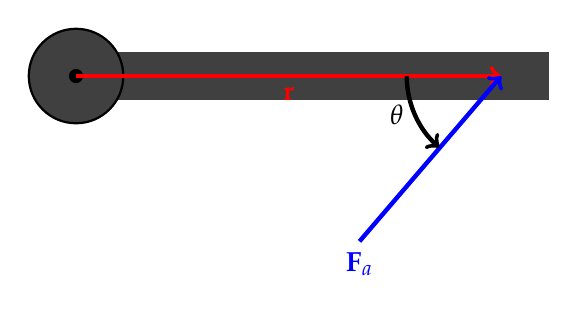
\begin{tikzpicture}[scale=3]
        \fill[black!75,draw=black!75] (0,-0.1) rectangle (2,0.1);
        \fill[black!75,draw=black,thick] (0,0) circle (.2);
        \fill[black] (0,0) circle (.03);
        \draw[ultra thick,red,->](0,0)--(1.8,0) node[midway,below]{$\mb{r}$};
        \draw[ultra thick,blue,->](1.2,-.7)--(1.8,0)node[pos=0,below]{$\mb{F}_a$};
        \draw[ultra thick,->] (1.4,0) arc(180:229:0.4)
        node[midway,left]{$\theta$};
      \end{tikzpicture}
    \end{center}
  \end{columns}
\end{frame}

\begin{frame}
  \frametitle{Vector Notation}
  In vector form, torque $\bm{\tau}$ is the cross product of the moment arm
  $\mb{r}$ and the applied force $\mb{F}_a$.

  \vspace{-0.2in}
  {\Huge
    \begin{displaymath}
      \boxed{\bm{\tau}=\mb{r}\times\mb{F}_a}
    \end{displaymath}
  }

  \vspace{-0.2in}
  \begin{center}
    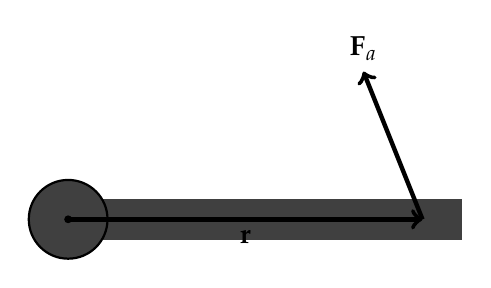
\begin{tikzpicture}[scale=2.5]
      \fill[black!75,draw=black!75] (0,-0.1) rectangle (2,0.1);
      \fill[black!75,draw=black,thick] (0,0) circle (.2);
      \fill[black] (0,0) circle (.02);
      \draw[ultra thick,->](0,0)--(1.8,0) node[midway,below]{$\mb{r}$};
      \draw[ultra thick,->](1.8,0)--(1.5,.75)node[pos=1,above]{$\mb{F}_a$};
    \end{tikzpicture}
  \end{center}
\end{frame}



\begin{frame}
  \frametitle{Torque (Moment)}
  Going back to the example question:
  \begin{center}
    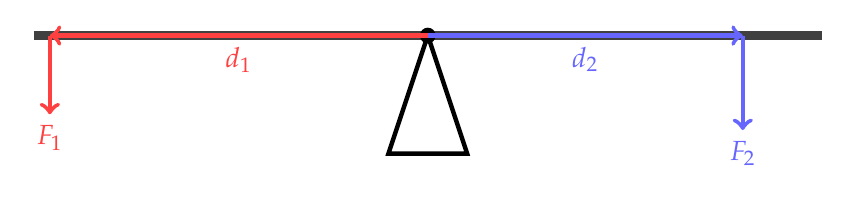
\begin{tikzpicture}
      \fill[black!75,draw=black!75] (-5,-0.05) rectangle (5,0.05);
      \fill (0,0) circle (.1);
      \draw[ultra thick](0,0)--(0.5,-1.5)--(-0.5,-1.5)--(0,0);
      \uncover<2->{
        \draw[ultra thick,red!75,->](0,0)--(-4.8,0) node[pos=.5,below]{$d_1$};
        \draw[ultra thick,red!75,->](-4.8,0)--(-4.8,-1)node[pos=1,below]{$F_1$};
      }
      \uncover<3->{
        \draw[ultra thick,blue!60,->](0,0)--(4,0) node[pos=.5,below]{$d_2$};
        \draw[ultra thick,blue!60,->](4,0)--(4,-1.2) node[pos=1,below]{$F_2$};
      }
    \end{tikzpicture}
  \end{center}
  \begin{itemize}
  \item<2-> $F_1$ will rotate the board counter clockwise
  \item<3-> $F_2$ will rotate the board clockwise
  \item<4-> The beam will remain static (in equilibrium) if

    \vspace{-0.2in}{\Large
    \begin{displaymath}
      F_1d_1=F_2d_2
    \end{displaymath}
  }
  \end{itemize}
\end{frame}


\begin{frame}
  \frametitle{Rotational Equilibrium}
  Just like \textbf{translational equilibrium} is when the force acting on an
  object is zero:
  
  \vspace{-0.35in}{\Large
    \begin{displaymath}
      \mb{F}=\mb{0}
    \end{displaymath}
  }

  \vspace{-0.1in}An object is in \textbf{rotational equilibrium} when the
  net torque acting on it is zero:

  \vspace{-0.2in}{\Large
    \begin{displaymath}
      \bm{\tau}=\mb{0}
    \end{displaymath}
  }

  \vspace{-0.1in}Note that it doesn't mean that the object isn't rotating, it
  just means that the object's rotational state isn't changing, i.e. $\alpha=0$
\end{frame}



\begin{frame}
  \frametitle{Example Problem}
  \textbf{Example 7a:} Find the net torque on point C.

  \vspace{-0.2in}\begin{center}
    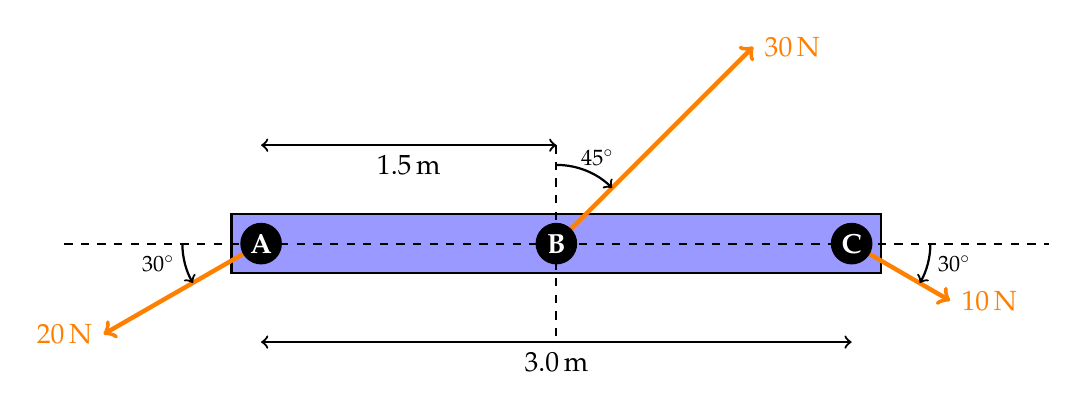
\begin{tikzpicture}[scale=2.5]
      \fill[blue!40!white,draw=black,thick] (-1.65,-0.15) rectangle (1.65,0.15);
      \draw[thick,<->](-1.5,-0.5)--(1.5,-0.5) node[midway,below]{\SI{3.0}{m}};
      \draw[thick,<->](-1.5,0.5)--(0,0.5) node[midway,below]{\SI{1.5}{m}};
      \draw[dashed,thick](-2.5,0)--(2.5,0);
      \draw[dashed,thick](0,.5)--(0,-.5);
      \draw[ultra thick,orange,->](0,0)--(1,1)node[pos=1,right]{\SI{30}{N}};
      \draw[thick,->](0,0.4)arc(90:45:0.4)
      node[pos=0.7,above]{\footnotesize\ang{45}};
      \draw[ultra thick,orange,->](-1.5,0)--(-2.3,-0.46)
      node[pos=1,left]{\SI{20}{\newton}};
      \draw[thick,->](-1.9,0) arc(180:210:0.4)
      node[midway,left]{\footnotesize\ang{30}};
      \draw[ultra thick,orange,->](1.5,0)--(2.0,-0.29)
      node[pos=1,right]{\SI{10}{\newton}};
      \draw[thick,->](1.9,0) arc(0:-30:0.4)
      node[midway,right]{\footnotesize\ang{30}};
      \fill[black,draw=black,thick] (-1.5,0) circle (0.1);
      \fill[black,draw=black,thick] (   0,0) circle (0.1);
      \fill[black,draw=black,thick] ( 1.5,0) circle (0.1);
      \node(A) at (-1.5,0) {\color{white}\textbf{A}};
      \node(B) at (0,0) {\color{white}\textbf{B}};
      \node(C) at (1.5,0) {\color{white}\textbf{C}};
    \end{tikzpicture}
  \end{center}
  \uncover<2->{
    \textbf{Example 7b:} Now find the net torque on A.
  }
\end{frame}



\section{Angular Momentum}

\begin{frame}
  \frametitle{Angular Momentum}
  \begin{columns}
    \column{.77\textwidth}
    Consider a mass $m$ connected to a massless beam rotates with speed $v$ at
    a distance $r$ from the center (shown on the right). It has an
    \textbf{angular momentum} ($L$) of
    
    \vspace{-0.25in}{\Large
      \begin{displaymath}
        \boxed{\mb{L}=\mb{r}\times\mb{p}}
      \end{displaymath}
    }
    
    \vspace{-0.15in}Expanding the terms in the definition:
    
    \vspace{-0.4in}{\Large
      \begin{displaymath}
        \mb{L}=\mb{r}\times(m\mb{v})=m\mb{r}\times(\bm{\omega}\times\mb{r})
        =mr^2\bm{\omega}
      \end{displaymath}
    }
    gives us:
    
    \vspace{-0.3in}{\Large
      \begin{displaymath}
        \boxed{\mb{L}=I\bm{\omega}}
      \end{displaymath}
    }
    The quantity $I$ is called the \textbf{moment of inertia}.
    \column{0.23\textwidth}
    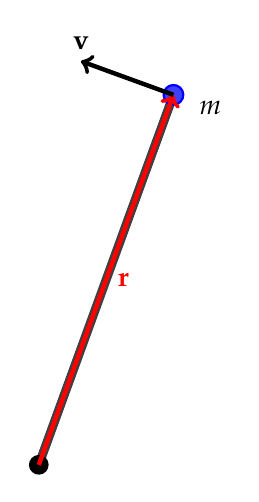
\begin{tikzpicture}[scale=2.5]
      \begin{scope}[rotate=70]
        \fill[black!75,draw=black!75] (0,-0.02) rectangle (2,0.02);
        \fill[blue!75,draw=blue,thick] (2,0) circle(.05);
        \node(M) at (2,-0.2) {$m$};
        \fill[black] (0,0) circle (.05);
        \draw[ultra thick,red,->](0,0)--(2,0)node[pos=.5,right]{$\mb{r}$};
        \draw[ultra thick,->](2,0)--(2,.5)node[pos=1,above]{$\mb{v}$};
      \end{scope}
    \end{tikzpicture}
  \end{columns}
\end{frame}


\begin{frame}
  \frametitle{Moment of Inertia}
  \begin{itemize}
  \item For a single particle:
    
    \vspace{-0.3in}{\Large
      \begin{displaymath}
        \boxed{I=r^2m}
      \end{displaymath}
    }
  \item A collection of particles:

    \vspace{-0.25in}{\Large
      \begin{displaymath}
        \boxed{I=\sum r_i^2m_i}
      \end{displaymath}
    }
  \item Continuous distribution of mass

    \vspace{-0.2in}{\Large
      \begin{displaymath}
        \boxed{I=\int r^2dm}
      \end{displaymath}
    }
  \end{itemize}
\end{frame}


\begin{frame}
  \frametitle{Moment of Inertia}
  \begin{center}
    \pic{.7}{mic.png}
  \end{center}
\end{frame}

\begin{frame}
  \frametitle{Angular Momentum and Moment of Inertia}
  \begin{itemize}
  \item Linear and angular momentum have very similar expressions
    
    \vspace{-0.25in}{\Large
      \begin{displaymath}
        \mb{p}=m\mb{v}\quad\quad\quad \mb{L}=I\bm{\omega}
      \end{displaymath}
    }
  \item Just like $\mb{p}$ describes the overall translational state of a
    physical system, $\mb{L}$ describes its overall rotational state
  \item In that case, momentum of inertia $I$ can be considered an object's
    ``rotational mass''
  \end{itemize}
\end{frame}



\begin{frame}
  \frametitle{Conservation of Angular Momentum}

  \vspace{-0.35in}{\Large
    \begin{displaymath}
      \bm{\tau}=\mb{r}\times\mb{F}=\mb{r}\times\frac{d\mb{p}}{dt}
      =\frac{d(\mb{r}\times\mb{p})}{dt}\;\;\longrightarrow\;\;
%      \tau=rF=rm\frac{dv}{dt}=\frac{d(rmv)}{dt}\quad\longrightarrow\quad
%    \end{displaymath}
%    \begin{displaymath}
      \boxed{\bm{\tau} =\frac{d\mb{L}}{dt}}
    \end{displaymath}
  }
  \begin{itemize}
  \item If the net torque on a system is zero, then the rate of change
    of angular momentum is zero, and we say that the angular momentum is
    conserved. 
  \item e.g.\ When an ice skater starts to spin and draws his arms inward.
    Since angular momentum is conserved, a decrease in $r$ means an
    increase in $\omega$.
  \item If moment of inertia $I$ is constant in time, the net torque is given
    by:

    \vspace{-0.2in}{\Large
      \begin{displaymath}
        \boxed{\bm{\tau}=I\bm{\alpha}}
      \end{displaymath}
    }
  \end{itemize}
\end{frame}


\begin{frame}
  \frametitle{Example Problem}
  \textbf{Example 8:} A skater extends her arms (both arms!), holding a
  \SI{2.0}{\kg} mass in each hand. She is rotating about a vertical axis at a
  given rate. She brings her arms inward towards her body in such a way that
  the distance of each mass from the axis changes from \SI{1.0}{\metre} to
  \SI{0.50}{\metre}. Her rate of rotation (neglecting her own mass) will?
\end{frame}


\begin{frame}
  \frametitle{Last Example}
  \textbf{Example 9:} A \SI{1}{\kg} mass swings in a vertical circle after
  having been released from a horizontal position with zero initial velocity.
  The mass is attached to a massless rigid rod of length \SI{1.5}{\metre}. What
  is the angular momentum of the mass, when it is in its lowest position?
\end{frame}


\section{Rotational Kinetic Energy}

\begin{frame}
  \frametitle{Rotational Kinetic Energy}
  To find the kinetic energy of a rotating system of particles (discrete number
  of particles, or continuous mass distribution), we can sum (or or integrate)
  the kinetic energy of the individual particles:
    
  \vspace{-0.3in}{\large
    \begin{align*}
      K&=\sum_i\frac{1}{2}m_iv_i^2=\frac{1}{2}\left(\sum_i m_ir_i^2\right)\omega^2\\
      K&=\int\frac{1}{2}v^2dm=\frac{1}{2}\left(\int r^2dm\right)\omega^2
    \end{align*}
  }
  
  \vspace{-0.15in}It's no surprise that in both case, rotational kinetic energy
  is given by:
  
  \vspace{-0.2in}{\Large
    \begin{displaymath}
      \boxed{K=\frac{1}{2}I\omega^2}
    \end{displaymath}
  }
\end{frame}


\begin{frame}
  \frametitle{Kinetic Energy of a Rotating System}
  The total kinetic energy of a rotating system is the sum of its translational
  and rotational kinetic energies at its center of mass:

  \vspace{-0.2in}{\Large
    \begin{displaymath}
      \boxed{K=\frac{1}{2}mv_\mathrm{CM}^2+\frac{1}{2}I_\mathrm{CM}\omega^2}
    \end{displaymath}
  }
  
  In this case, $I_\mathrm{CM}$ is calculated at the center of mass. For simple
  problems, we only need to compute rotational kinetic energy at the pivot:

  \vspace{-0.2in}{\Large
    \begin{displaymath}
      \boxed{K=\frac{1}{2}I_\mathrm{P}\omega^2}
    \end{displaymath}
  }
  
  In this case, the $I_\mathrm{P}$ is calculated at the pivot.
  \textbf{IMPORTANT:} $I_\mathrm{CM}\neq I_\mathrm{P}$
\end{frame}
%\begin{frame}
%  \frametitle{Linear vs.\ Angular Motion}
%  \begin{center}
%    \begin{tabular}{c|l|l}
%      & Linear & Angular\\\hline
%      Equation of Motion &
%      $\displaystyle \mb{F}_\mathrm{net}=\frac{d\mb{p}}{dt}=m\mb{a}$ &
%      $\displaystyle \bm{\tau}=\mb{F}\times\mb{r}=\frac{d\mb{L}}{dt}=I\alpha$\\
%      Momentum & $\mb{p}=m\mb{v}$ & $\mb{L}=m\mb{v}\times\mb{r}$\\
%      Kinetic Energy & $\displaystyle K=\frac{1}{2}mv^2$ &
%      $\displaystyle K=\frac{1}{2}I\omega^2$ \\
%      \end{tabular}
%  \end{center}
%\end{frame}

\end{document}
